%%%%%%%%%%%%%%%%%%%%%%%%%%%%%%%%%%%%%%%%%%%%%%%%%%%
%                                                 %
%                     SECTION                     %
%                                                 %
%%%%%%%%%%%%%%%%%%%%%%%%%%%%%%%%%%%%%%%%%%%%%%%%%%%

\section{Tasks}
\label{sec:sec007}

During our user tests, we need to ask participants to provide a subjective assessment of their experience using our \textit{Assistant}. There are several widely used questionnaires giving us different prons-and-cons. However, in most cases, a \hyperlink{https://www.nngroup.com/articles/keep-online-surveys-short/}{single question instrument}~\cite{sauro201210} is the right method for a quantitative usability testing. By taking less time and effort to answer, participants are pursuing to this phase after task, while it is minimally disruptive.

\clearpage

The tasks were derived from test scenarios ({\it i.e.}, {\bf Sce1.} and {\bf Sce2.}) developed from use cases and/or with the assistance of a subject-matter expert.  Due to the range and extent of functionality provided in the system, and the short time for which each participant will be available, the tasks are the most common and relatively complex for the available functions. The tasks are identical for all participants of a given user role in the study.

At this stage, each participant will interact with our UI. The UI show to each participant the set of patients chosen randomly (Section \ref{sec:sec001}). The set of patients will provide participants with 50 patients, while all patients much have at least one of the three available modalities (Figure \ref{fig:svmm}). Each participant will open each patient ({\it e.g.}, {\bf Pat1.}, {\bf Pat2.} or {\bf Pat3.}), of the three patients chosen randomly, and will examine the set of images. During examination, the participant will interact with the available features (Section \ref{sec:sec005}) of the system.

%%%%%%%%%%%%%%%%%%%%%%%%%%%%%%%%%%%%%%%%%%%%%%%%%%%

\hfill

\begin{wrapfigure}{r}{0.50\textwidth}
\centering
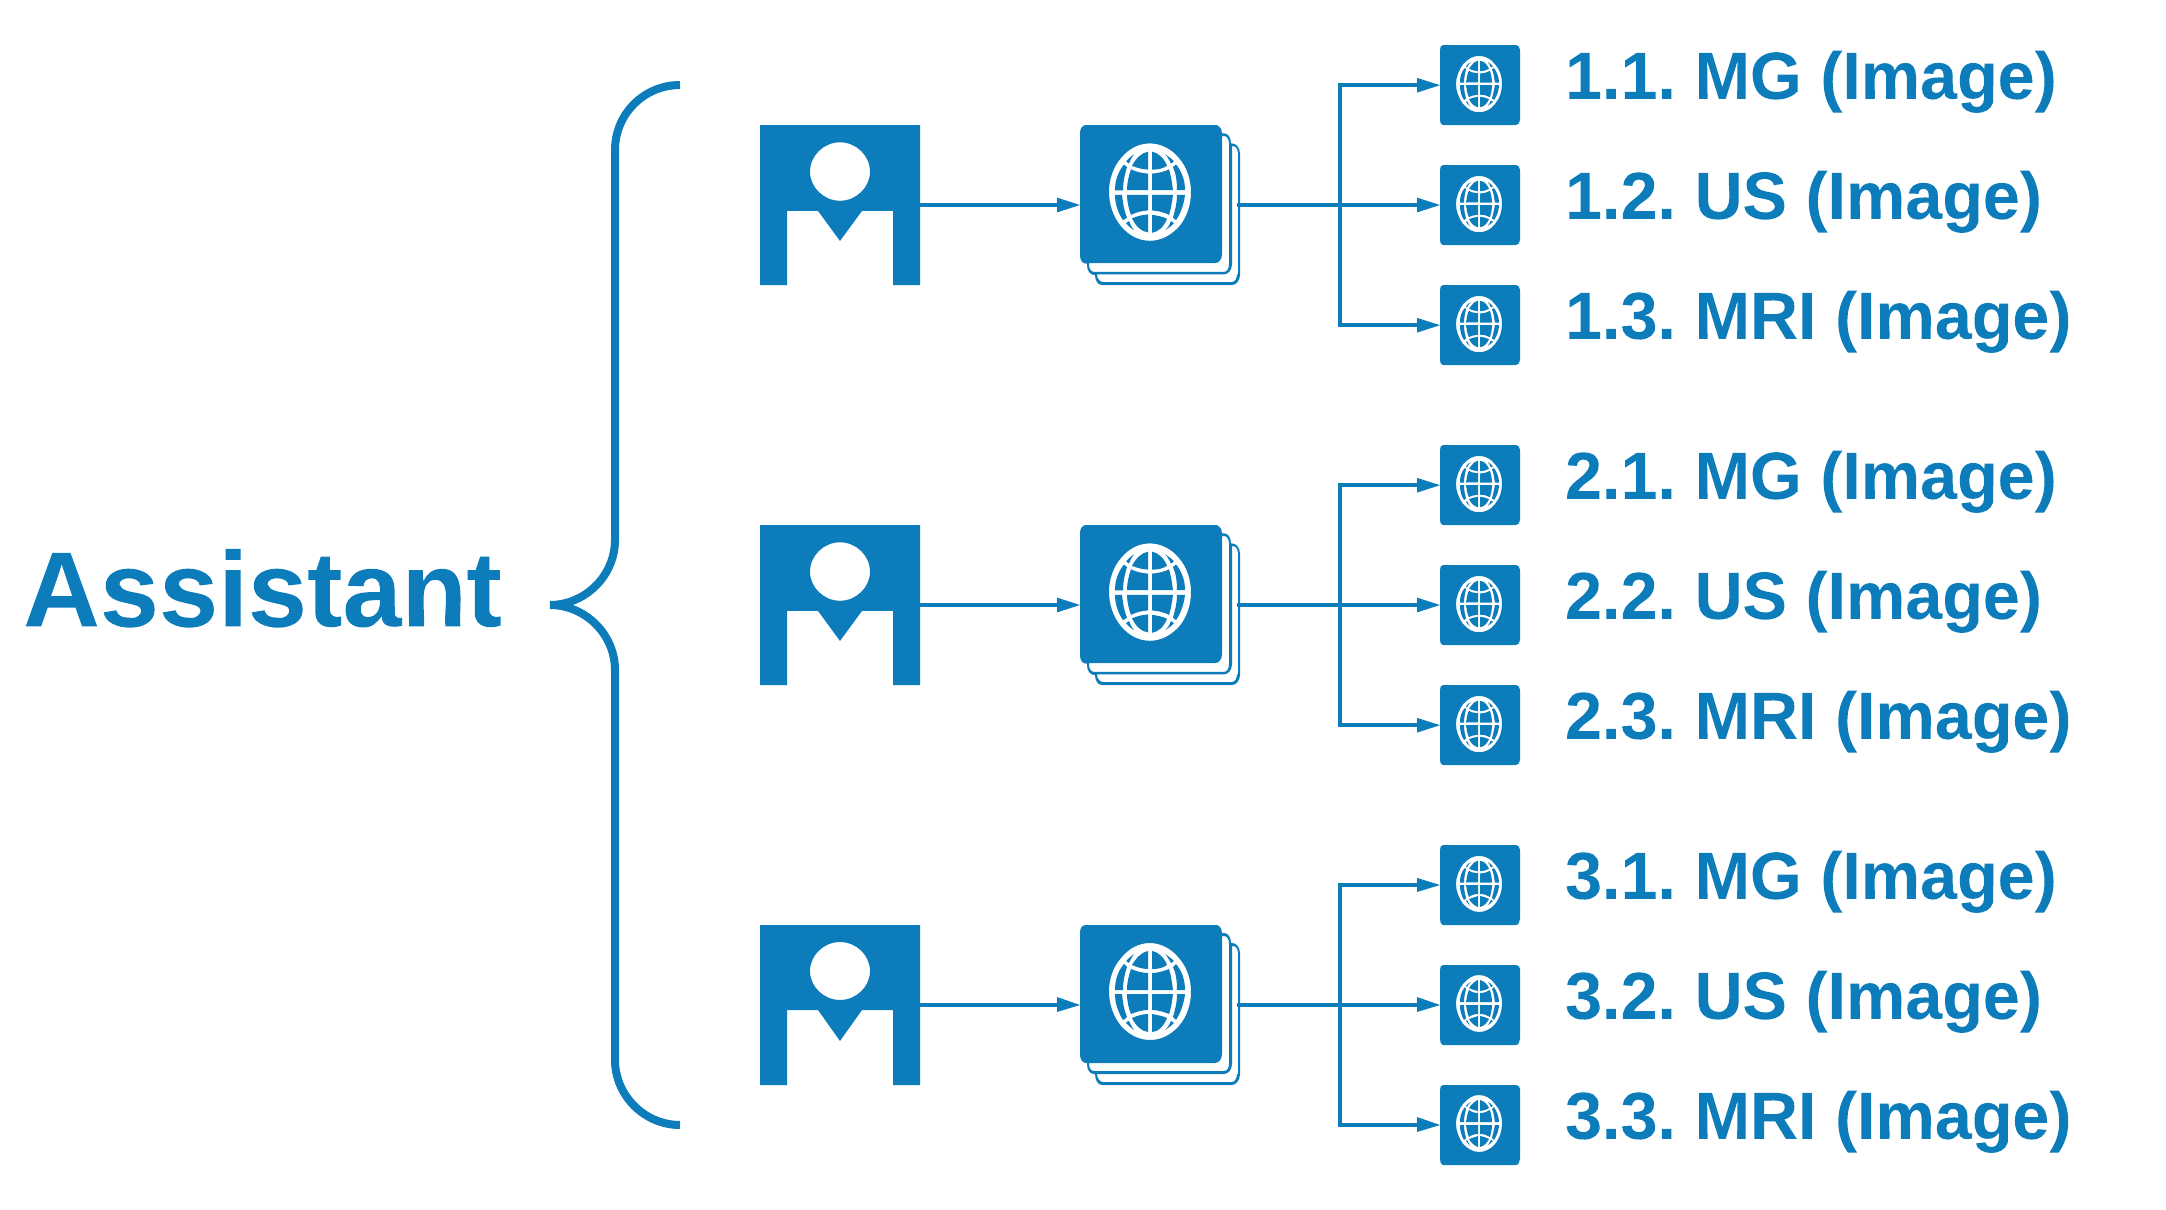
\includegraphics[width=0.50\textwidth]{img001}
\caption{Diagram representing the use of the \textit{Assistant} by clinicians.}
\label{fig:svmm}
\end{wrapfigure}

\hfill

%%%%%%%%%%%%%%%%%%%%%%%%%%%%%%%%%%%%%%%%%%%%%%%%%%%

We will try to understand if, with the \textit{AI-Assisted} techniques, the clinicians will encounters the most accurate severity (\hyperlink{https://en.wikipedia.org/wiki/BI-RADS}{BIRADS}) of the breast lesions~\cite{american1998breast} and patient's prognostic. For this purpose, we have three patients (Figure \ref{fig:svmm}); each patient has three images in the respective modalities: (i) MG; (ii) US; and (iii) MRI. The clinicians will proceed to the activity of diagnosing the three patients within the support of our \textit{Assistant} by the observation of all images.

\hfill

In our \textit{User Testing Guide} a set of tasks is necessary and carefully crafted. Our test studies involve asking participants to perform a set of tasks. By looking at what our user need to do with our system, our tasks are realistic as possible. We are not describing the exact steps participants need to take. We achieve that by avoiding the precise language used as labels in our system. The tasks are emotionally neutrals. And we did several \hyperlink{https://www.nngroup.com/articles/pilot-testing/}{pilot tests} to prevent misleading situations saving us from wasting resources by accidentally use a lousy task or from getting bad data. The tasks are as follows.

The task descriptions below are required to be reviewed by all researchers and facilitators (Section \ref{sec:sec004}) to ensure that the content, format, and presentation are representative of real use and substantially evaluate the total system. Their acceptance is to be documented prior to the user test. Each task, is related to the set of {\it Phases}, {\it Scenarios} and {\it Activities} (Section \ref{sec:sec001}) on the next section (Section \ref{sec:sec008}) further explained.

\clearpage

%%%%%%%%%%%%%%%%%%%%%%%%%%%%%%%%%%%%%%%%%%%%%%%%%%%

List of stand alone tasks for both {\bf Pha1.}, {\bf Pha2.} and {\bf Pha3.} phases:

%%%%%%%%%%%%%%%%%%%%%%%%%%%%%%%%%%%%%%%%%%%%%%%%%%%

\hfill

\begin{itemize}
\item[] \textbf{Task 1.1.1:} Fill the Consent Form (Section \ref{sec:sec001}) and accept the user test;
\item[] \textbf{Task 1.1.2:} Fill the User Characterization Form (Section \ref{sec:sec001}) and proceed;
\end{itemize}

\hfill

\begin{itemize}
\item[] \textbf{Task 2.1.1:} Classify \textit{Patient 1} ({\bf Pat1.}) on the \textit{MM} condition;
\item[] \textbf{Task 2.1.2:} Classify \textit{Patient 2} ({\bf Pat2.}) on the \textit{MM} condition;
\item[] \textbf{Task 2.1.3:} Classify \textit{Patient 3} ({\bf Pat3.}) on the \textit{MM} condition;
\end{itemize}

\hfill

\begin{itemize}
\item[] \textbf{Task 2.2.1:} Freely explore \textit{Patient 1} ({\bf Pat1.}) on the \textit{MM} condition;
\item[] \textbf{Task 2.2.2:} Freely explore \textit{Patient 2} ({\bf Pat2.}) on the \textit{MM} condition;
\item[] \textbf{Task 2.2.3:} Freely explore \textit{Patient 3} ({\bf Pat3.}) on the \textit{MM} condition;
\end{itemize}

\hfill

\begin{itemize}
\item[] \textbf{Task 2.3.1:} Workload \& Usability questions for the \textit{MM} condition;
\item[] \textbf{Task 2.3.2:} {\it Post-task} questions for the \textit{MM} condition;
\end{itemize}

\hfill

\begin{itemize}
\item[] \textbf{Task 3.1.1:} Classify \textit{Patient 1} ({\bf Pat1.}) on the \textit{Assis.} condition;
\item[] \textbf{Task 3.1.2:} Classify \textit{Patient 2} ({\bf Pat2.}) on the \textit{Assis.} condition;
\item[] \textbf{Task 3.1.3:} Classify \textit{Patient 3} ({\bf Pat3.}) on the \textit{Assis.} condition;
\end{itemize}

\hfill

\begin{itemize}
\item[] \textbf{Task 3.2.1:} Freely explore \textit{Patient 1} ({\bf Pat1.}) on the \textit{Assis.} condition;
\item[] \textbf{Task 3.2.2:} Freely explore \textit{Patient 2} ({\bf Pat2.}) on the \textit{Assis.} condition;
\item[] \textbf{Task 3.2.3:} Freely explore \textit{Patient 3} ({\bf Pat3.}) on the \textit{Assis.} condition;
\end{itemize}

\hfill

\begin{itemize}
\item[] \textbf{Task 3.3.1:} Workload \& Usability questions for the \textit{Assis.} condition;
\item[] \textbf{Task 3.3.2:} {\it Post-task} questions for the \textit{Assis.} condition;
\end{itemize}

\hfill

%%%%%%%%%%%%%%%%%%%%%%%%%%%%%%%%%%%%%%%%%%%%%%%%%%%